
\section{Community Support Study (RQ1)}
\label{communitystudy}
The goal of this study is to understand how frequently each of the regex representations appears in source code. Based on the results, we identify preferred representations using popularity in source code.



\subsection{Artifacts}
To determine how common each regex representations is in the wild, we collected
regexes from GitHub projects. We specifically targeted Python projects as it is a popular programming language with a strong presence on GitHub. Further, Python is the fourth most common language on GitHub (after Java, Javascript and Ruby) and Python's regex pattern
language is close enough to other regex libraries that our conclusions are likely to generalize.

We collected and analyzed static invocations to the Python {\tt re} library.
Figure~\ref{fig:exampleUsage} presents an example  from Python  with key components labeled. The \emph{function} called is {\tt re.compile}.
The \emph{pattern} defines what strings will be matched and the \emph{flag} {\tt re.MULTILINE} modifies the rules used by the regex engine when matching.
When executed, a regex object {\tt r1} is created
%The regex pattern is an ordered series of regular expression language feature tokens.
and it will  match if it finds a zero at the end of a line, or a (possibly negative) integer at the end of a line (i.e., due to the {\tt -?} sequence denoting zero or one instance of the {\tt -}).

\begin{figure}[tb]
\centering
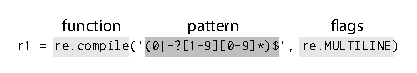
\includegraphics[width=\columnwidth]{refactoring/illustrations/exampleUsage.eps}
\vspace{-12pt}
\caption{Example of one regex library invocation}
\vspace{-6pt}
\label{fig:exampleUsage}
\end{figure}

Our goal was to collect regex patterns from a variety of projects to represent the breadth of how developers use regexes.
We scraped 3,898 projects containing Python code using the GitHub API. This was done by systematically selecting repository IDs, checking the repository for Python files, and retaining the project if Python was found. After dividing eight million repository IDs into 32 groups, we scanned from the beginning until we had collected approximately four thousand Python projects.
%We did so  by dividing a range of about 8 million repo IDs
%into 32 sections of equal size and scanning  for Python projects from the beginning of those
%segments until we ran out of memory.
At that point, we felt we had enough data
to do an analysis without further perfecting our mining techniques.

To identify invocations of the {\tt re} module, we built
the AST of each Python file in each project. In most projects, almost all {\tt re} invocations are present in the
most recent version of a project, but to be more thorough, we also scanned up
to 19 earlier versions.
%The number 20 was chosen to try and maximize returns on
%computing resources invested after observing the scanning process in many hours
%of trial scans.
% If the project had fewer than 20 commits, then all commits were scanned.
% The most recent commit was always included, and the spacing between all other chosen commits was determined by dividing the remaining number of commits by 19 (rounding as needed).
All regex patterns were obtained, sans duplicates.
%Within a project, a duplicate utilization was marked when two versions of the same file have the same function, pattern and flags.
In the end, we observed and recorded 16,088 non-duplicate patterns in 1,645 projects.
%\todoLast{1544 may be a white lie...the 13K+ patterns come from 1544 projects, but the 54k utilizations (before pruning) probably come from something like 1900 projects, and that number is somewhere in the git history of tour de source}

In collecting the set of distinct patterns for analysis,  we ignore the 12.7\%  of {\tt re} invocations using flags, which can alter regex behavior.  An additional 6.5\% of {\tt re} invocations contained patterns that could not be compiled because the pattern was non-static (e.g., used some runtime variable).
%The remaining 80.8\% (43,525) of the utilizations were collapsed into 13,711 distinct pattern strings.
This parser was unable to support 0.8\% (114) due to error.
% of the patterns due to unsupported unicode characters.  Another 0.2\% (25) of the patterns used regex features that we  chose to exclude because they appeared very rarely (e.g., reference conditions).  An additional 0.1\% (16) of the patterns were excluded because they were empty or otherwise malformed so as to cause a parsing error.
After removing all problematic patterns as described and collapsing on duplicates, we ended up with 13,597 distinct patterns from 1,544 projects remained to be used in this study.



\subsection{Metrics}
\label{sec:communitymetric}
We measure community support by matching each regex in the corpus to the representations (nodes) in Figure~\ref{fig:refactoringTree} and counting the number of \emph{patterns} that contain the representation and the number of \emph{projects} that contain the representation.
%A \emph{pattern} is extracted from a utilization, as shown in Figure~\ref{fig:exampleUsage}.
Note that a regex can belong to multiple representations, and a regex can belong to multiple projects since we collapsed duplicates and only analyze the distinct regex patterns.
% that represent 43,525 regex utilizations across the projects.\todoMid{feels weird to hear this again right away, maybe simplify the metrics paragraph}
%For this frequency analysis, we focus on patterns and the number of projects the patterns appear in.
%To determine how often each representation appears in the wild, we extract regex patterns from source code and measure if a representation matches (part of) the pattern.
%
%
%\paragraph{Patterns}



%\paragraph{Projects}

%The process for deciding if a particular pattern belongs to a particular node is described in detail in Section~\ref{communityanalysis}.





\subsection{Analysis}
\label{communityanalysis}
To determine how many of the representations match patterns in the corpus, we performed an analysis using the PCRE parser and by representing the regexes as token streams, depending on the characteristics of the representation. Our analysis code is available on GitHub\footnote{\url{https://github.com/softwarekitty/regex_readability_study}}. Next, we describe the process in detail:

\subsubsection{Presence of a Feature}
For the representations that only require a particular feature to be present, such as the question-mark in D2, the features identified by the PCRE parser were used to decide membership of patterns in nodes.
These feature-requiring nodes are as follows: D1 requires double-bounded repetition with different bounds, D2 requires the question-mark repetition, S1 requires single-bounded repetition, S3 requires double-bounded repetition with the same bounds,  L1 requires a lower-bound repetition, L2 requires the kleene star (\verb!*!) repetition, L3 requires the add (\verb!+!) repetition, and C3 requires a negated custom character class.

\subsubsection{Features  and Pattern}
For some representations, the presence of a feature is not enough to determine membership.
However,  the presence of a feature and properties of the pattern can determine membership.


Identifying D3 requires an OR containing at least two entries - some sequence present in one entry repeated N times, and then the same sequence present in another entry repeated N+1 times.  This is a hard pattern to detect directly, but we identified candidates by looking for a sequence of N repeating groups with an OR-bar (ie. \verb!|!) next to them on one side (either side).  This produced a list of 113 candidates which we narrowed down manually to 10 actual members.


Identifying T2 requires a literal feature that matches the regex \verb!(\\x[a-f0-9A-F]{2})! which reliably identifies hex codes within a pattern.
Similarly T4 requires a literal feature and must match the regex \verb!((\\0\d*)|(\\\d{3}))! which is specific to Python-style octal, requiring either exactly three digits after a slash, or a zero and some other digits after a slash.  Only one false positive was identified which was actually the lower end of a hex range using the literal \verb!\0!.

Identifying T3 requires that a single literal character is wrapped in a custom character class (a member of T3 is always a member of C2).
 T1 requires that no characters are wrapped in brackets or are hex or octal characters, which actually matches over 91\% of the total patterns analyzed.

\subsubsection{Token Stream }
The following representations were identified by representing the regex patterns as a sequence of dot-delimited tokens.
Identifying S2 requires any element to be repeated at least twice. This element could be a character class, a literal, or a collection of things encapsulated in parentheses.
Identifying C1 requires that a non-negative character class contains a range.  Identifying C2 requires that there exists a custom character class that does not use ranges or defaults. Identifying C4 requires the presence of a default character class within a custom character class, specifically, \verb!\d!, \verb!\D!, \verb!\w!, \verb!\W!, \verb!\s!, \verb!\S! and \verb!.!.  Identifying C5 requires an OR of length-one sequences (literal characters or any character class).


\subsection{Results}
Table~\ref{table:nodeCount} presents the frequencies with which each representation appears in a regex pattern and in a project scraped from GitHub. The \emph{node} column references the representations in Figure~\ref{fig:refactoringTree} and the \emph{description} column briefly describes the representation, followed by an \emph{example} from the corpus. The \emph{nPatterns} column counts the patterns that belong to the representation, followed by the percent of patterns out of 13,597.
The \emph{nProjects} column counts the projects that contain a regex belonging to the representation,
followed by the percentage of projects out of 1,544.
Recall that the patterns are all unique and could appear in multiple projects, hence the project support is used to show how pervasive the representation in across the whole community.
For example, 2,479 of the patterns belong to the C1 representation, representing 18.2\% of the patterns. These appear in 810 projects, representing 52.5\%.
 Representation D1 appears in 346 (2.5\%) of the patterns but only 234 (15.2\%) of the projects. In contrast, representation T3 appears in 39 \emph{fewer} patterns but 34 \emph{more} projects, indicating that D1 is more concentrated in a few projects and T3 is more widespread across projects.

Using the pattern frequency as a guide, we can create refactoring recommendations based on community frequency. For example, since C1 is more prevalent than C2, we could say that C2 is smelly since it could better conform to the community standard if expressed as C1. Thus, we might recommend a $\overrightarrow{C2C1}$ refactoring. Based on patterns alone, the winning representations per equivalence class are C1, D2, T1, L2, and S2. With one exception, these are the same for recommendations based on projects. The difference is that L3 appears in more projects than L2, so it is not clear which is more desirable based on community standards.
Section~\ref{sec:rq3} explores these results more deeply.

%Table~\ref{summaryResults} presents these recommendations for each pair of representations within each equivalence class. The \emph{Comm} column is populated based on the findings of \emph{RQ1}. The findings for \emph{RQ2} and \emph{RQ3} are in the \emph{Match} and \emph{Compose} columns, respectively.
